\newpage

{%
\footnotesize
\textit{Uwaga: przytoczone fragmenty mogą być luźną interpretacją relacji podanego autora.}
}

\DeclareRobustCommand{\wioslo}{%
  \begingroup\normalfont%
  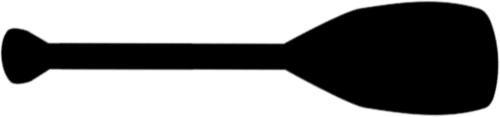
\includegraphics[height=0.8\fontcharht\font`\B]{images/wioslo.png}%
  \endgroup
}

\newcounter{notka}[section]
\newenvironment{notka}[2]{
    \refstepcounter{notka}
    \def\tytul{#1}
    \def\autor{#2}
    \bigskip
    \Large \wioslo{} \hspace{0.2cm} \tytul{}
    \normalsize
    \bigskip

    \begin{adjustwidth}{1cm}{1cm}
}{
    \end{adjustwidth}
    \hfill{} \autor{}
}

\begin{notka}{Śpiewanie na wodzie}{Ola Gawryła}
    Magia mórz, oceanów i innych mniejszych, większych oraz pośrednich
    akwenów wodnych zawierających ciekłe \ce{H2O} powoduje, że każdy
    nagle śpiewa pięknie, nikt nie fałszuje i możemy się tylko
    zachwycać swoimi cudownymi głosami.
\end{notka}

\begin{notka}{Koszt sprzętów na wodzie}{Kapitan Kamil}
    Na wodzie wszystko jest dużo droższe. To jest ogólny aksjomat, który
    za chwilę sobie wyprowadzimy, natomiast możesz pewnie skojarzyć,
    że na stacji benzynowej również jest dwa razy drożej --- to prawda,
    jednak warunkach marynistycznych skala problemu jest znacznie większa. Spójrzmy na
    następujące fakty i liczby:
    \begin{itemize}
        \item Listwa drewniana $35 \times 35 \times 1000$ mm w Lerła --- 11,00 zł
        \item Bosak drewniany 210 cm w sklepie żeglarskim --- 168,00 zł
    \end{itemize}
    Na chłopski rozum spodziewalibyśmy się, że taki dwumetrowy
    bosak będzie kosztował kilka złotych z hakiem, skoro bez haka wychodzi
    dwa złote. Jednak okazuje się, że taki zdroworozsądkowy
    szacunek należy przemnożyć razy 100, a czasem 1000, aby uzyskać
    koszt danego sprzętu w zastosowaniu na wodzie. Myślisz, że taki
    kręciołek od lin zwany przez fanatyków \say{kabestanem} na pewno
    nie kosztuje więcej, niż paręnaście złotych, co? Zastanów się jeszcze~raz\ldots
\end{notka}

